\documentclass[10pt]{article}
\usepackage[a4paper, margin=2cm]{geometry}
%\usepackage{fullpage}
\usepackage[T1]{fontenc}
\usepackage[utf8]{inputenc}
\usepackage{graphicx}
\usepackage{mathpazo}
\pagenumbering{arabic}
\usepackage{siunitx}
\usepackage{amsmath}
\usepackage{mathtools} % Para poder usar "\Aboxed"
\usepackage{cancel} % Para usar "\cancel", de https://tex.stackexchange.com/questions/537955/how-do-cross-out-text-in-math-mode
\usepackage{multicol}
\usepackage[spanish]{babel}
\usepackage{steinmetz}
\DeclareSIUnit\voltampere{VA}
\DeclareSIUnit\var{VA_r}
\setlength\parindent{0pt} % no indent

% Numbering pages on the right footer:
% (https://tex.stackexchange.com/questions/153167/how-to-set-page-number-at-right-footer)
\usepackage{fancyhdr}
% Turn on the style
\pagestyle{fancy}
\fancyhf{} % sets both header and footer to nothing
\renewcommand{\headrulewidth}{0pt} % To remove the top horizontal line created by default by "fancyhdr", from here: https://tex.stackexchange.com/questions/13896/how-to-remove-the-top-horizontal-bar-in-fancyhdr
% Set the right side of the footer to be the page number
\fancyfoot[R]{\thepage}


\usepackage{minibox} % Para poder partir el texto en 2 líneas usando "underbrace" u "overbrace", info aquí: https://tex.stackexchange.com/questions/8680/how-can-i-insert-a-newline-in-a-framebox


\usepackage{xparse} % For "overbrace/underbrace but with an arrow instead", from https://tex.stackexchange.com/questions/8720/overbrace-underbrace-but-with-an-arrow-instead

% Para poner flechas sobre los signos de igual, de aquí: https://tex.stackexchange.com/questions/8720/overbrace-underbrace-but-with-an-arrow-instead
\NewDocumentCommand{\overarrow}{O{=} O{\uparrow} m}{%
  \overset{\makebox[0pt]{\begin{tabular}{@{}c@{}}#3\\[0pt]\ensuremath{#2}\end{tabular}}}{#1}
}
\NewDocumentCommand{\underarrow}{O{=} O{\downarrow} m}{%
  \underset{\makebox[0pt]{\begin{tabular}{@{}c@{}}\ensuremath{#2}\\[0pt]#3\end{tabular}}}{#1}
}





\begin{document}

\large{\textbf{Enunciado}}:

\vspace{3mm}
Un generador cuya \textit{fem} es de \qty{120}{\volt} y resistencia de \qty{0.2}{\ohm}, da una corriente de \qty{20}{\ampere} a un motor situado a \qty{300}{\meter} de distancia y de resistencia \qty{0.5}{\ohm}. La línea que los conecta es de cobre, de resistividad \qty{17.24}{\milli\ohm\milli\meter\squared\per\meter}. Sabiendo que el motor absorbe \qty{10.2}{\kWh} en \qty{5}{\hour}, se debe hallar:
\vspace{3mm}

\begin{enumerate}
    \item La fuerza contraelectromotriz (\textit{fcem}) del motor
    \item La sección de los conductores de la línea
    \item Los rendimientos de: motor, generador, línea y rendimiento total
    \item El balance general de potencias
\end{enumerate}


\hrulefill

\vspace{5mm}
\textbf{Solución}:
\vspace{4mm}

Empezamos dibujando el esquema del circuito y organizando los datos disponibles:
\vspace{6mm}

\begin{minipage}{0.73\linewidth}
  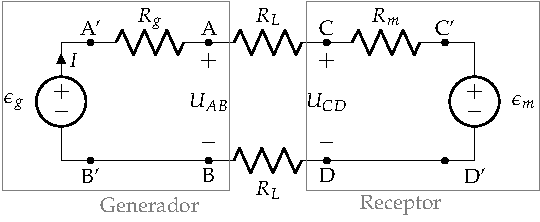
\includegraphics[scale=1.25]{figs/circuito_lkv.pdf}
\end{minipage}
\begin{minipage}{0.27\linewidth}
  \textbf{Datos}:
  \vspace{2mm}
  
  $\epsilon_g = \qty{120}{\volt}$\\
  $R_g = \qty{0.2}{\ohm}$\\
  $I = \qty{20}{\ampere}$\\
  $R_m = \qty{0.5}{\ohm}$\\
  $E_m = \qty{10.2}{\kWh}$ (en $\qty{5}{\hour}$)\\
  $l = \qty{300}{\meter}$\\
  $\rho = \qty{17.24}{\milli\ohm\milli\meter\squared\per\meter}$
\end{minipage}

\vspace{6mm}

Donde la resistencia de la línea se divide en dos elementos, para distinguir entre el conductor de aporte y el de retorno de corriente.

\vspace{6mm}

\underline{Apartado 1}

\vspace{4mm}

Para calcular $\epsilon_m$, podemos formular el balance de tensiones (2LK) en la parte del motor:
\[
  U_{CD} = \underbrace{I \cdot R_m}_{= 20 \cdot 0.5} + \epsilon_m
\]

Pero para despejar $\epsilon_m$ en la expresión anterior, necesitamos calcular $U_{CD}$.
\begin{itemize}
    \item Opción 1: aplicar el balance de tensiones en la ``parte izquierda'' del circuito (a la izquierda de $U_{CD}$ en el diagrama). 
    
    \underline{Problema}: no conocemos el valor de $R_L$ (y no podemos calcularlo usando la resistividad, porque desconocemos la sección de los conductores), luego no podemos calcular la caída de tensión en la línea.
    
    \item Opción 2: leyendo de nuevo la información que tenemos sobre el punto de operación del motor, vemos que es conocida la potencia absorbida por este.

    \[
      P_{CD} = \frac{10.2 \cdot 10^{-3} \, \si{\kWh}}{\qty{5}{\hour}} = \qty{2040}{\watt}
    \]

    Luego:
    \[
      P_{CD} = U_{CD} \cdot I \quad \rightarrow \quad U_{CD} = \frac{2040}{20} = \qty{102}{\volt}
    \]

    Sustituyendo en la primera expresión:
    \[
      \epsilon_m = U_{CD} - 10 = \boxed{ \qty{92}{\volt} }
    \]

    \item Opción 3 (forma alternativa de llegar al resultado anterior): aplicar balance de potencias en el motor.
    \[
      P_{\textrm{útil}} = P_{\textrm{absorbida}} - P_{\textrm{pérdidas}} \quad \rightarrow \quad P_{\epsilon_m} = P_{CD} - \hspace{-6mm} \underbrace{P_{R_m}}_{\substack{= R_m \cdot I^2 \\[3pt] \text{(ley de Joule)}}}
    \]
    
    $P_{CD}$ se calcula de la forma descrita en la Opción 2, luego $P_{\epsilon_m}$ se obtiene como:
    \[
      P_{\epsilon_m} = 2040 - 0.5 \cdot 20^2 = \qty{1840}{\watt}
    \]

    Finalmente: 
    \[
      P_{\epsilon_m} = \epsilon_m \cdot I \quad \rightarrow \quad \epsilon_m = \frac{1840}{20} = \boxed{ \qty{92}{\volt} }
    \]
\end{itemize}

\vspace{3mm}

\underline{Apartado 2}

\vspace{5mm}

Para calcular la sección de la línea:
\[
  R_L = \rho \cdot \frac{l}{S} = {17.24 \cdot 10^{-3}}\si{\ohm\milli\meter\squared\per\meter} \cdot \frac{\qty{300}{\meter}}{S}
\]
(dado que ambos conductores, tanto el de aporte como el de retorno de corriente, tienen una $l=\qty{300}{\meter}$ cada uno)

\vspace{3mm}    
Luego debemos calcular el valor de $R_L$ para poder despejar $S$.
\begin{itemize}
    \item Opción 1: aplicar el balance de tensiones en todo el circuito (2LK). Comenzando en el punto $A$, y retornando al mismo punto:
    
    \[
      R_L \cdot I + U_{CD} + R_L \cdot I - \epsilon_g + R_g \cdot I = 0
    \]
    Despejando $R_L$:
    \[
      2 R_L \cdot I = \underbrace{\epsilon_g}_{=\qty{120}{\volt}} - \underbrace{R_g \cdot I}_{=0.2 \cdot 20} - \underbrace{U_{CD}}_{=\qty{102}{\volt}} \quad \rightarrow \quad \boxed{ R_L = {\frac{7}{20}}\si{\ohm} }
    \]

    \item Opción 2: aplicar balance de potencias en la línea.

    \vspace{2mm}
    \begin{minipage}{0.4\linewidth}
    \begin{center}
      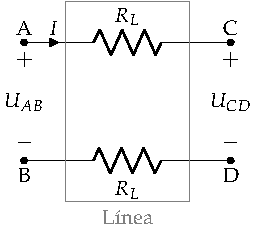
\includegraphics[scale=1.2]{figs/linea_lkv.pdf}
    \end{center}
    \end{minipage}
    \begin{minipage}{0.6\linewidth}
    \begin{align*}
        P_{\textrm{entrada}} &= P_{\textrm{pérdidas línea}} + P_{\textrm{salida}}\\[10pt]
        U_{AB} \cdot I &= 2 \cdot R_L \cdot I^2 + U_{CD} \cdot I\\[10pt] 
        R_L &= \frac{U_{AB}-U_{CD}}{2 \cdot I} \underarrow[=][\uparrow]{\small 2LK para \ensuremath{U_{AB}} } \frac{\epsilon_g - I\cdot R_g - 102}{2 \cdot 20} = \Aboxed{ {\frac{7}{20}}\si{\ohm} }
        % Flecha, sacada de aquí: https://tex.stackexchange.com/questions/8720/overbrace-underbrace-but-with-an-arrow-instead
        % Sin "\ensuremath" da error al meter un símbolo matemático
    \end{align*}
    \end{minipage}
\end{itemize}

Una vez conocemos el valor de $R_L$, despejamos $S$ en la primera expresión:

\[
  S = \rho \cdot \frac{l}{R_L} = \boxed{ \qty{14.78}{\milli\meter\squared} }
\]

Dado que este valor no corresponde a una sección normalizada de cable, en la práctica este circuito contendría un cable de sección normalizada inmediatamente superior a este valor, es decir, de $S = \qty{16}{\milli\meter\squared}$.

\vspace{6mm}

\underline{Apartado 3}

\vspace{5mm}

Los rendimientos pedidos se calculan de la siguiente forma:
\begin{align*}
    \eta_m &= \frac{P_{\textrm{útil}}}{P_{\textrm{absorbida}}} = \frac{\epsilon_m \cdot \bcancel{I}}{U_{CD} \cdot \bcancel{I}} = \frac{\qty{92}{\volt}}{\qty{102}{\volt}} \hspace{22mm} = \rlap{\kern-0.5ex\fbox{\rule[-2.5pt]{0pt}{12pt}\rule{27pt}{0pt}}} 0.902\\[10pt]
    \eta_g &= \frac{P_{\textrm{entregada}}}{P_{\textrm{producida}}} = \frac{U_{AB}}{\epsilon_g} = \frac{\qty{116}{\volt}}{\qty{120}{\volt}} \hspace{26.1mm}= \rlap{\kern-0.5ex\fbox{\rule[-2.5pt]{0pt}{12pt}\rule{27pt}{0pt}}} 0.967\\[10pt]
    \eta_{\textrm{línea}} &= \frac{P_{\textrm{salida}}}{P_{\textrm{entrada}}} = \frac{U_{CD}}{U_{AB}} = \frac{\qty{102}{\volt}}{\qty{116}{\volt}} \hspace{29.5mm} = \rlap{\kern-0.5ex\fbox{\rule[-2.5pt]{0pt}{12pt}\rule{27pt}{0pt}}} 0.879\\[10pt]
    \eta_{\textrm{total}} &= \frac{P_{\textrm{útil}}}{P_{\textrm{producida}}} = \frac{\epsilon_m}{\epsilon_g} = \frac{\qty{92}{\volt}}{\qty{120}{\volt}} = \eta_g \cdot \eta_{\textrm{línea}} \cdot \eta_g = \rlap{\kern-0.5ex\fbox{\rule[-2.5pt]{0pt}{12pt}\rule{27pt}{0pt}}} 0.767
\end{align*}
% Uso "\rlap" porque, por alguna razón, "\Aboxed" mueve los resultados muy a la derecha. Idea para usar "\rlap" sacada de aquí: https://tex.stackexchange.com/questions/223511/aboxed-with-multiple-in-align-environment

\vspace{6mm}

\underline{Apartado 4}

\vspace{5mm}

El balance de potencias del circuito es:

\[
  P_{g} = P_{\textrm{línea}} + P_{m} 
\]

Donde:

\begin{align*}
    P_{g} &= P_{\textrm{útil}, \, g} + P_{\textrm{pérdidas}, \, g} &\rightarrow  \qquad &\epsilon_g \cdot I = U_{AB} \cdot I + R_g \cdot I^2 \\[10pt]
    P_{\textrm{línea}} &= P_{\textrm{útil, línea}} + P_{\textrm{pérdidas, línea}} \hspace{-20mm} &\rightarrow \qquad &U_{AB} \cdot I = U_{CD} \cdot I + 2 R_L \cdot I^2\\[10pt]
    P_{m} &= P_{\textrm{útil}, \, m} + P_{\textrm{pérdidas}, \, m} &\rightarrow  \qquad &U_{CD} \cdot I = \epsilon_m \cdot I + R_m \cdot I^2 
\end{align*}


\end{document}

